\section{Methodology}
\label{sec:methodology}

\subsection{Obfuscation Testing Protocol}

The core innovation of our methodology is temporal obfuscation---systematically removing temporal and contextual information while preserving structural market mechanics. The protocol involves five transformations:

\begin{enumerate}
\item Convert absolute dates (``2024-01-16'') to relative format (``Day T+0'')
\item Replace ticker symbols (``SPY'') with generic identifiers (``INDEX\_1'')
\item Remove market events (``Fed meeting'', ``earnings'')
\item Strip volatility regime context (``VIX at 14'')
\item Eliminate day-of-week patterns (``Monday'', ``OpEx Friday'')
\end{enumerate}

Preserved information includes: net gamma exposure values, directional gamma (calls vs.\ puts), spot price and flip point levels, relative time progression, and concentration metrics. Fig.~\ref{fig:obfuscation} illustrates this transformation.

\begin{figure}[!htbp]
\centering
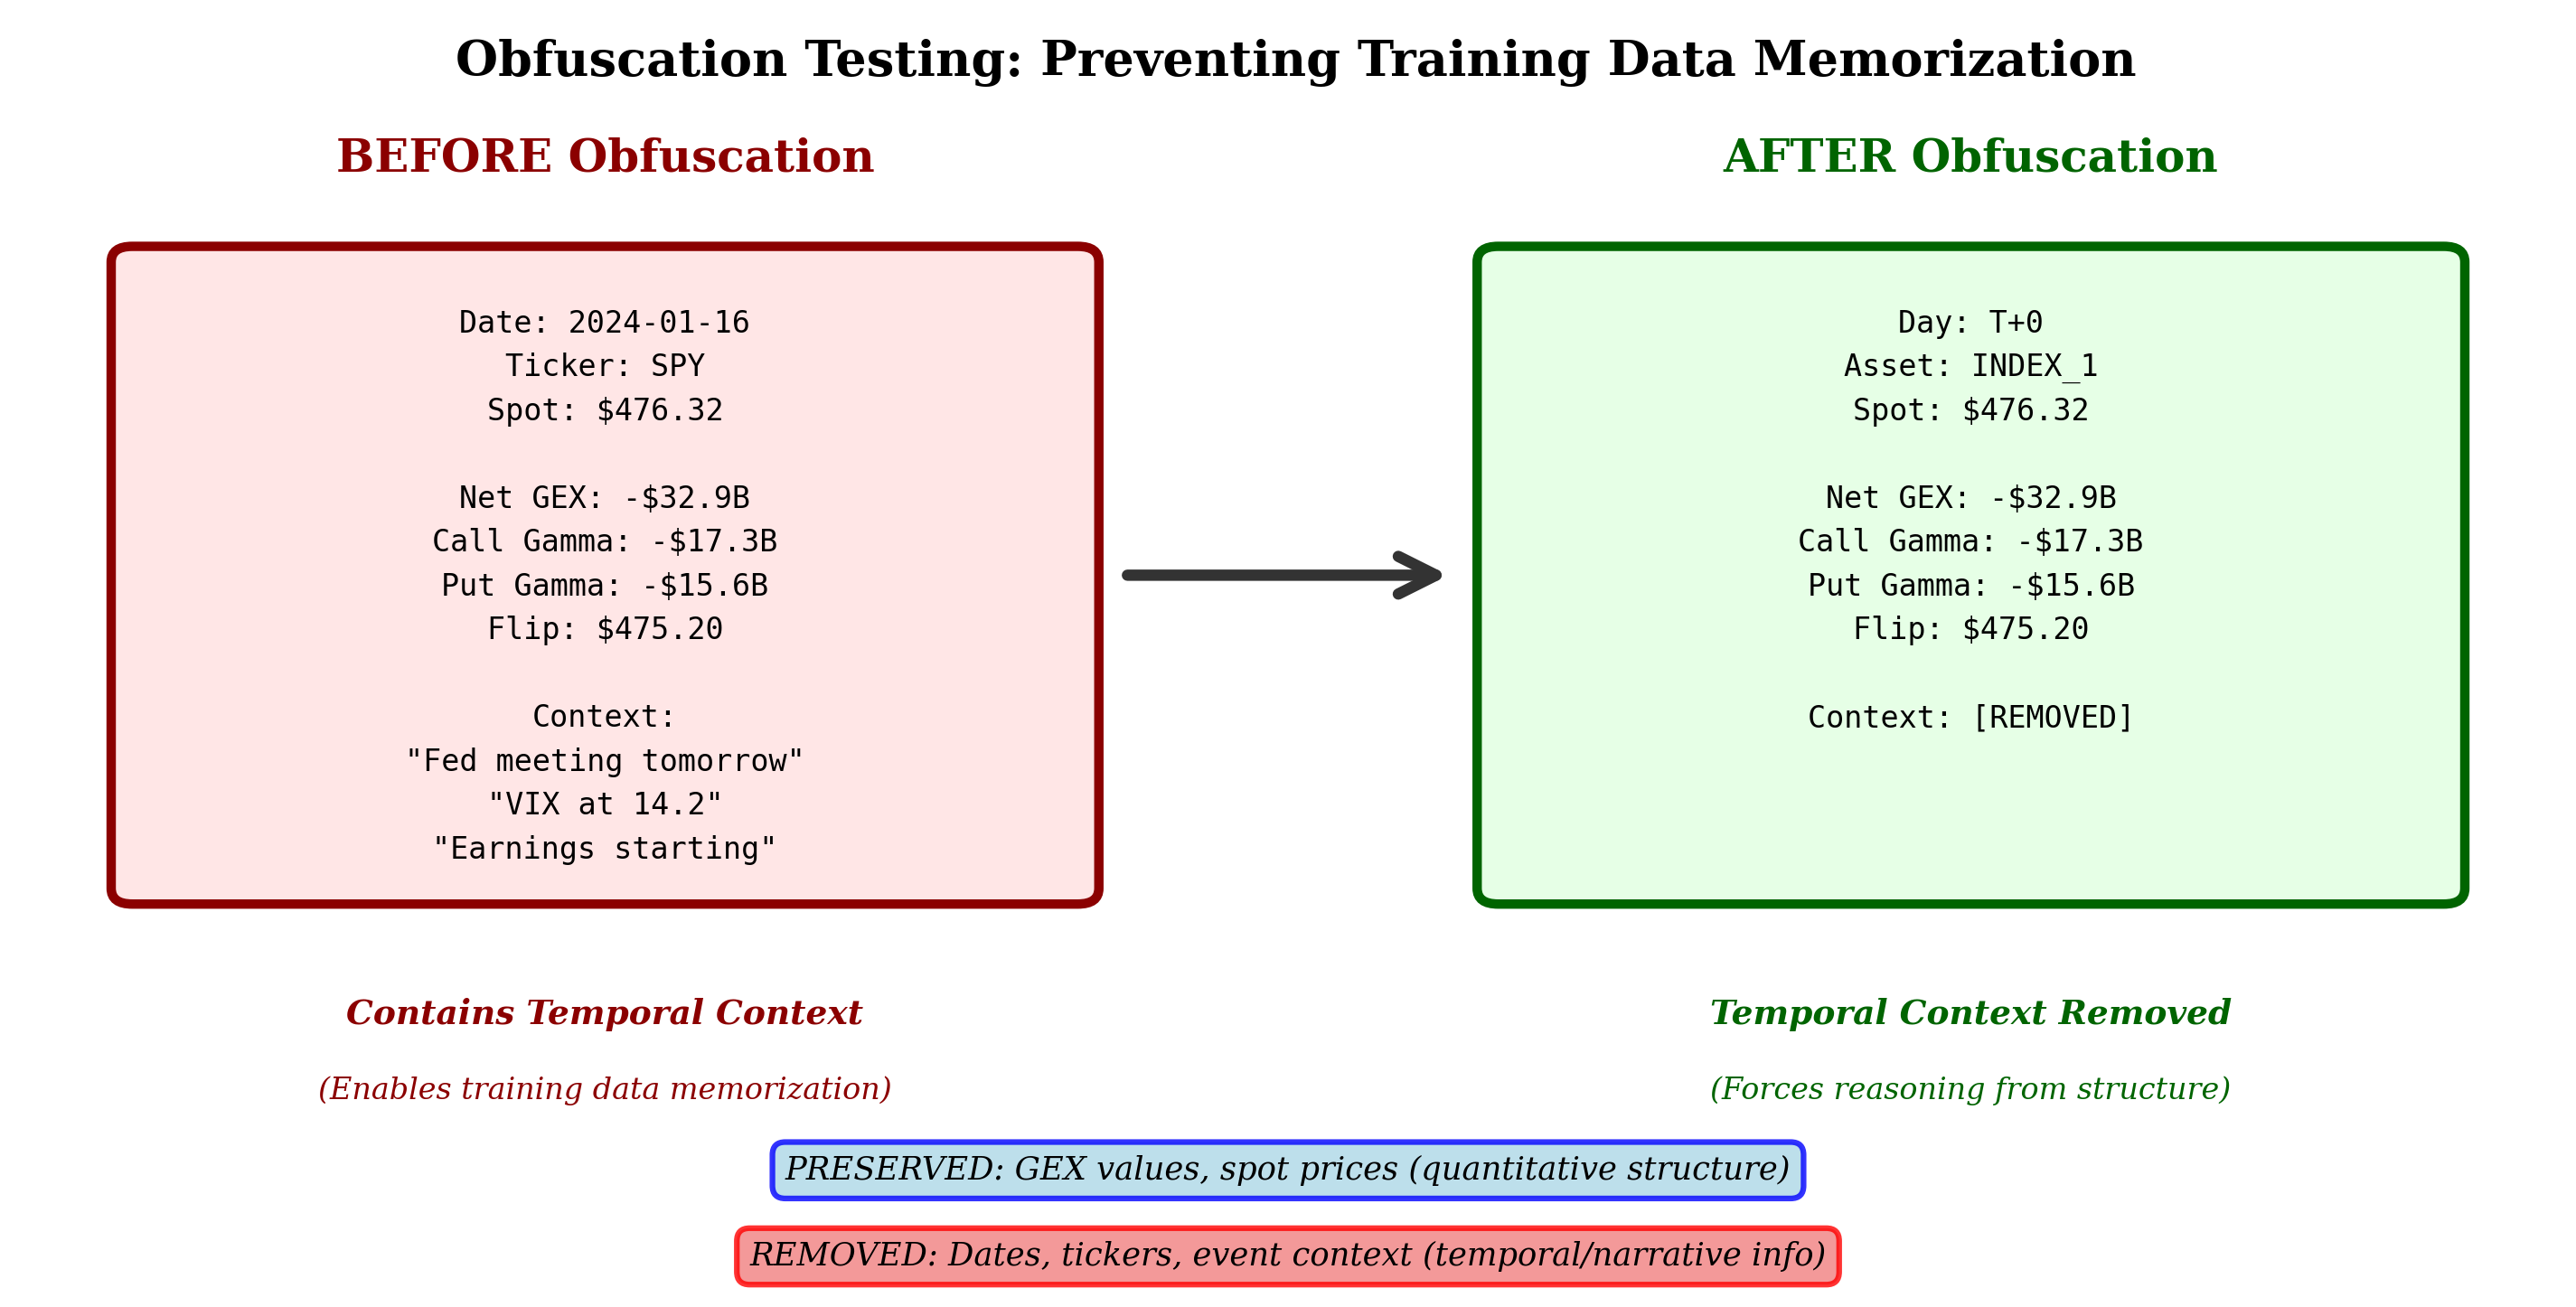
\includegraphics[width=\columnwidth]{figures/fig01_obfuscation_example.png}
\caption{Temporal obfuscation methodology. Left: Original data with dates, ticker symbols, and market context. Right: Obfuscated data preserving only structural quantitative relationships.}
\label{fig:obfuscation}
\end{figure}

As a concrete example, the transformation converts raw market data:

\begin{small}
\begin{verbatim}
SPY, 2024-03-15: Net GEX: -$32.9B, Flip: $485.00
SPY, 2024-03-18: Net GEX: -$28.4B, Flip: $487.50
\end{verbatim}
\end{small}

\noindent into obfuscated format:

\begin{small}
\begin{verbatim}
Day T+0, INDEX_1: Net GEX: -$32.9B, Flip: $485.00
Day T+1, INDEX_1: Net GEX: -$28.4B, Flip: $487.50
\end{verbatim}
\end{small}

The quantitative values are identical; only contextual identifiers change. This approach forces LLMs to identify patterns from quantitative relationships alone. A model memorizing ``January 2024 SPY negative gamma'' cannot succeed when presented with ``Day T+0 INDEX\_1 GEX: -\$32B''. Only genuine structural understanding enables detection under these conditions.

\subsection{Causal Framework: WHO$\rightarrow$WHOM$\rightarrow$WHAT}

Beyond detecting patterns, we require models to articulate causal mechanisms:

\textbf{WHO}: The economic actor with structural constraints (e.g., ``dealers with negative gamma exposure'').

\textbf{WHOM}: The affected market participants (e.g., ``directional traders and market makers'').

\textbf{WHAT}: The forced action and mechanism (e.g., ``must sell rallies and buy dips to maintain delta neutrality, amplifying volatility'').

This framework, derived from agent-based market microstructure theory~\cite{grossman1988liquidity,garleanu2009demand}, prevents vague pattern claims and requires specific mechanical understanding. It implements a structured form of chain-of-thought prompting~\cite{wei2022chain}, ensuring the model derives outcomes from mechanical constraints rather than recalling historical correlations.

A valid causal chain demonstrates the complete mechanism. For example: WHO---``Dealers accumulate net short gamma exposure of \$28B concentrated at the 520 strike.'' WHOM---``Market makers holding these positions are forced to continuously delta-hedge to maintain regulatory neutrality.'' WHAT---``As price rises toward 520, dealers must buy shares to offset negative delta, amplifying the upward move; as price falls, they must sell, amplifying downward moves. This creates a pro-cyclical feedback loop that persists until gamma exposure dissipates.'' The causal chain must connect actors to mechanisms to observable outcomes, preventing the model from declaring patterns without articulating the structural logic that produces them.

\subsection{Single-Day Pattern Detection}
\label{subsec:single_day_method}

To ensure robustness, we test three narrative framings of the same underlying dealer constraint (Table~\ref{tab:patterns}). All reflect the same structural reality---dealers hedging option exposure---but use different conceptual lenses. Consistent detection across framings validates genuine understanding rather than keyword matching.

\begin{table}[!htbp]
\centering
\caption{Three Pattern Framings of Dealer Hedging Constraints}
\label{tab:patterns}
\small
\begin{tabular}{@{}lccc@{}}
\toprule
\textbf{Pattern} & \textbf{Framing} & \textbf{WHO} & \textbf{WHAT} \\
\midrule
Gamma Positioning & Technical/Greek & Dealers with $-\Gamma$ & Pro-cyclical hedging \\
Stock Pinning & Behavioral & Market makers & Strike convergence \\
0DTE Hedging & Temporal & Option writers & Rapid rebalancing \\
\bottomrule
\end{tabular}
\end{table}

We establish three validation levels: (1) detection rate $\geq$60\% (exceeds random chance), (2) prediction accuracy $\geq$80\% (forward returns match), and (3) correct WHO$\rightarrow$WHOM$\rightarrow$WHAT specification $\geq$90\%.

\subsection{30-Day Regime Detection Framework}

Extending from single-day patterns, we define \textit{persistent regimes} through three structural criteria applied to rolling 30-day windows. Each window contains 30 consecutive trading days of GEX values, generated with stride 1 (producing $N - 29$ overlapping windows from $N$ trading days). Windows are labeled ``Day T$-$29'' through ``Day T+0'' to preserve relative temporal ordering while removing absolute date information. For each year, this generates approximately 220 windows from $\sim$250 trading days, yielding the 1,412 real windows across 2020--2025 used in our analysis.

We classify each window using three structural criteria:

\textbf{Persistence}: Fraction of days sharing the dominant GEX sign.
\begin{equation}
P = \frac{\text{days with dominant sign}}{30} \geq 0.70
\end{equation}

\textbf{Magnitude}: Average absolute gamma exposure.
\begin{equation}
M = \frac{1}{30}\sum_{i=1}^{30} |\text{GEX}_i| \geq \$5\text{B}
\end{equation}

\textbf{Stability}: Maximum sign flips across 30 days.
\begin{equation}
S = \text{count}(\text{sign}(\text{GEX}_{i+1}) \neq \text{sign}(\text{GEX}_i)) \leq 5
\end{equation}

Windows meeting all three criteria are classified as persistent regimes (positive or negative); others are transitional or low-conviction. The \$5B magnitude threshold reflects dealer risk management practices, while 70\% persistence ensures directional bias significantly exceeds random binomial variation ($\approx 2.2\sigma$). Fig.~\ref{fig:regime_window} illustrates an example persistent regime.

\begin{figure}[!htbp]
\centering
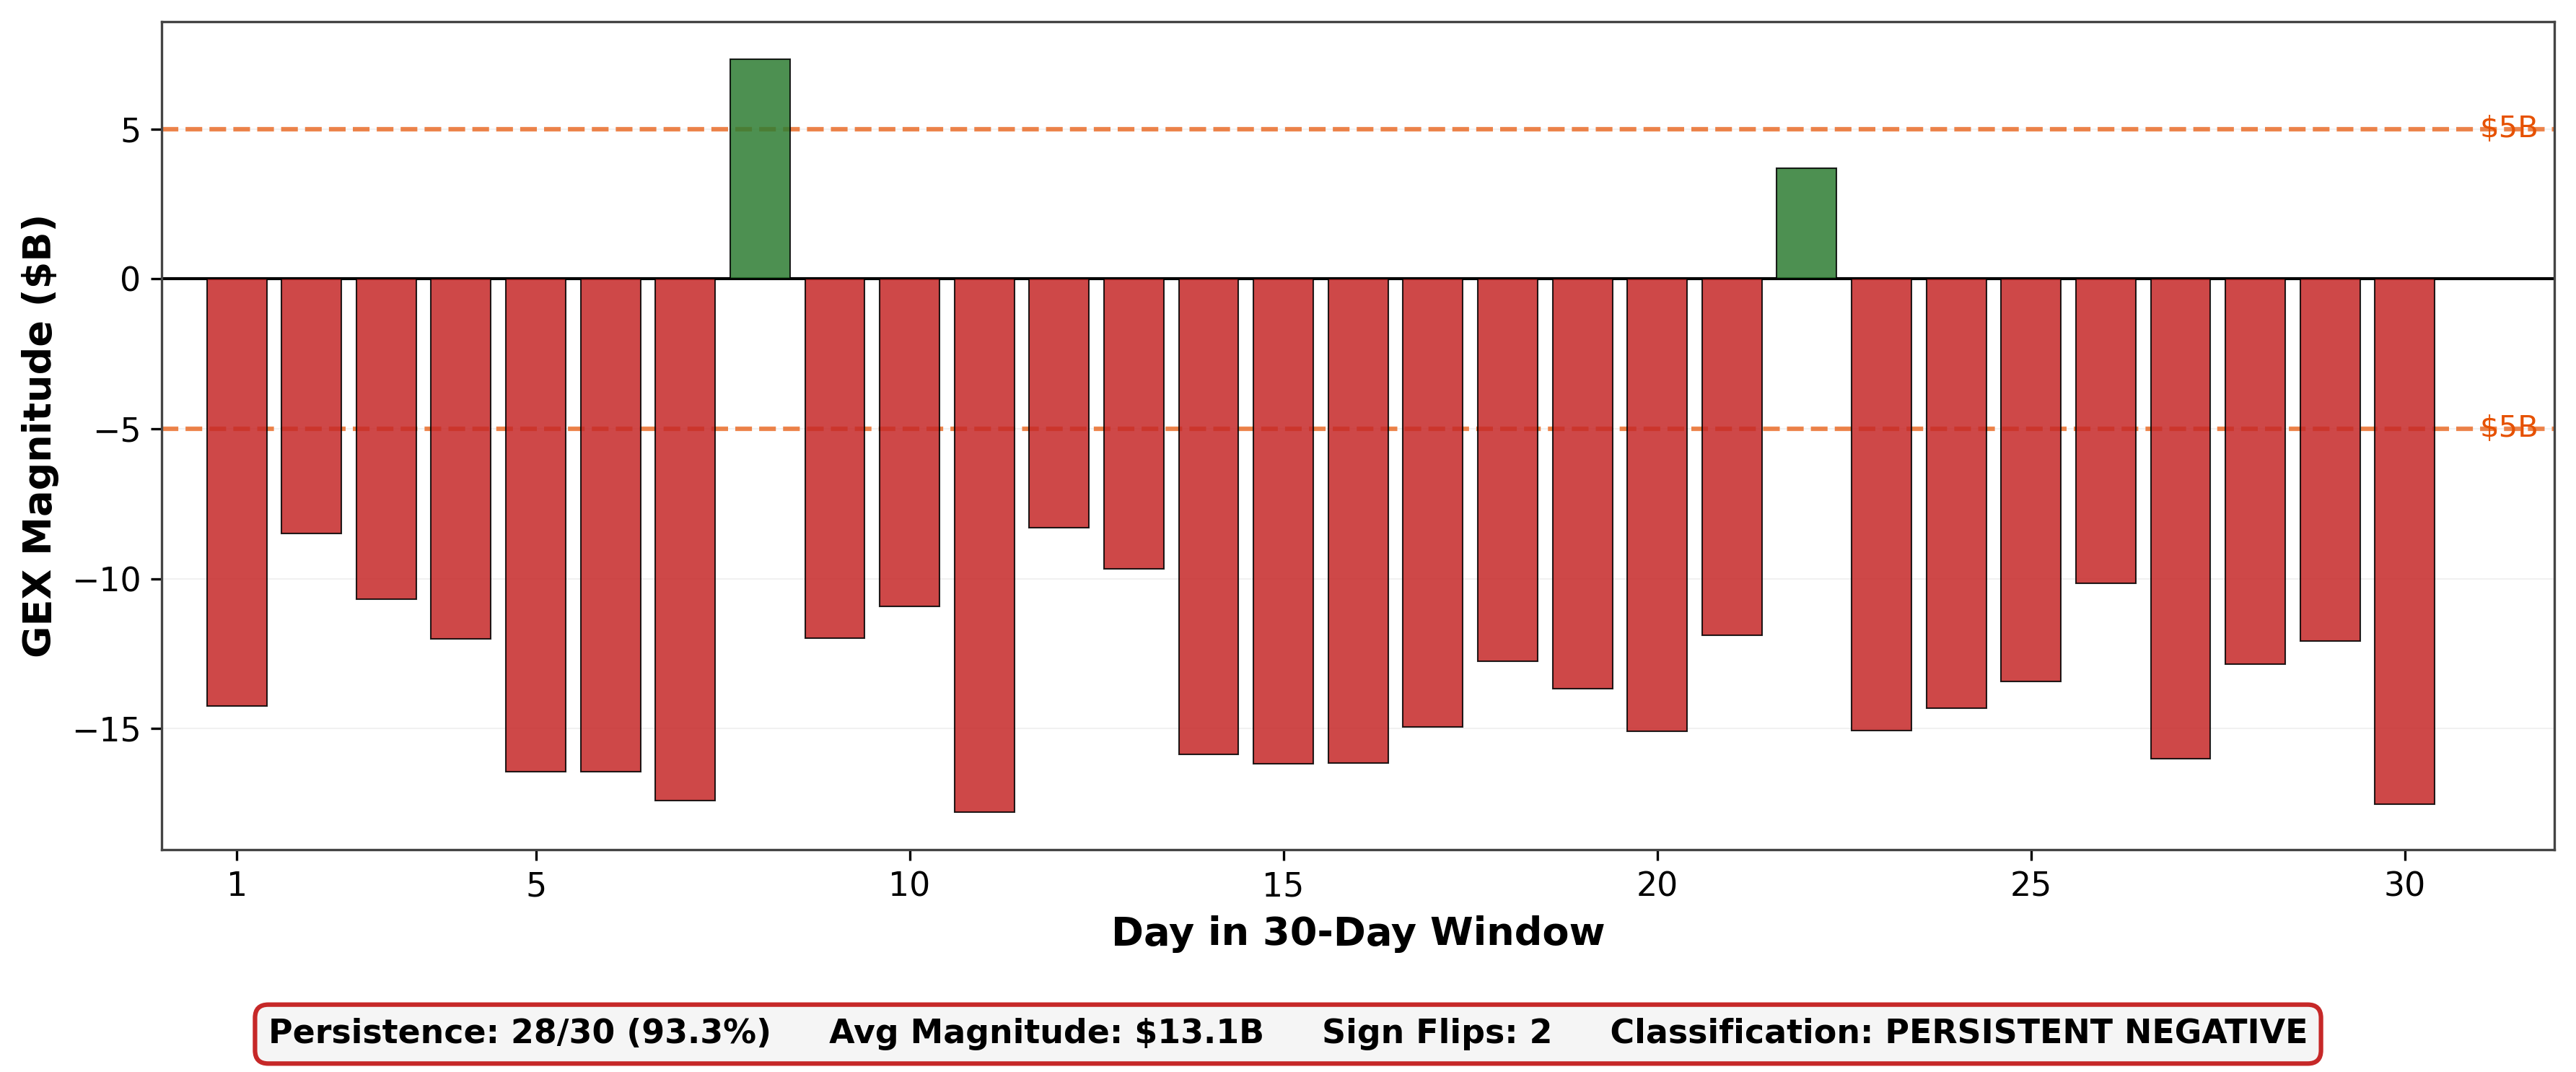
\includegraphics[width=\columnwidth]{figures/fig08_regime_window.png}
\caption{30-day persistent negative regime example. Daily GEX values showing 28/30 days negative (93.3\% persistence), average magnitude \$14.1B, and only 2 sign flips.}
\label{fig:regime_window}
\end{figure}

\subsection{GEX Calculation}

Following standard market microstructure practice~\cite{anderegg2022impact,spotgamma2021}, we calculate dealer gamma exposure from end-of-day open interest:

\begin{equation}
\text{GEX} = \sum_i \pm \text{OI}_i \times \Gamma_i \times S^2 \times 0.01 \times 100
\end{equation}

where $\Gamma_i$ is the Black-Scholes gamma~\cite{black1973pricing,hull2018options} at strike $i$, $\text{OI}_i$ is open interest, $S$ is the underlying spot price, and the $S^2$ factor scales gamma to dollar exposure (since gamma measures $\partial^2 V / \partial S^2$, multiplying by $S^2$ produces dollar-denominated sensitivity). The sign convention reflects the dealer counterparty relationship: calls contribute positive GEX (dealers are typically long gamma on calls) and puts contribute negative GEX (dealers are typically short gamma on puts)~\cite{anderegg2022impact}.

The resulting aggregate GEX value has a direct mechanical interpretation. \textbf{Positive GEX} indicates dealers are net long gamma: they buy when prices fall and sell when prices rise, \textit{dampening} volatility. \textbf{Negative GEX} indicates dealers are net short gamma: they sell when prices fall and buy when prices rise, \textit{amplifying} volatility through pro-cyclical hedging flows. The magnitude determines the scale of forced hedging---a $-$\$20B GEX day implies larger rebalancing flows than a $-$\$5B day, though our Granger causality analysis (Section~\ref{subsec:granger}) reveals a threshold effect: the \textit{presence} of negative gamma drives volatility amplification, not the specific level.

This open interest-based approach (GEX\_OI) measures dealer inventory positioning rather than intraday flow. While volume-based GEX may better capture 0DTE dynamics, 30-day window aggregation smooths daily measurement noise, and the underlying hedging mechanism remains constant regardless of measurement method~\cite{dim2025zero}.

We deliberately constrain analysis to gamma rather than higher-order Greeks (vanna, charm). Gamma hedging represents a universal regulatory requirement binding across institutions~\cite{mixon2009}, making it the ideal testing ground where all participants face the same fundamental constraint. Higher-order Greeks vary across proprietary implementations, precluding objective ``ground truth'' validation.

\subsection{Multi-Phase Validation Strategy}

For regime detection, we employ a five-phase protocol spanning 2020--2025:

\textbf{Phase 1} (Q1 2024 Baseline, 52 windows): Establish baseline detection rate. Success criteria: 30--50\% (demonstrates selectivity, not universal matching).

\textbf{Phase 2} (Negative Controls, 809 windows): Three synthetic control types, each violating a specific regime criterion:
\begin{itemize}
    \item \textit{Shuffled} (404 windows): Randomize day order within real windows, destroying temporal structure while preserving aggregate statistics. Tests whether detection depends on temporal ordering or merely aggregate distribution.
    \item \textit{Transitional} (202 windows): Generate windows with frequent sign flips ($>$8 per window), violating the stability criterion. Tests whether the model incorrectly classifies volatile positioning as persistent regimes.
    \item \textit{Low-magnitude} (203 windows): Generate windows with magnitude below \$3B, violating the magnitude criterion. Tests whether the model flags weak positioning as economically meaningful.
\end{itemize}
Expected: $<$10\% false positive rate across all control types.

\textbf{Phase 3} (Full 2024, 223 windows): Test Q1 generalization across all 252 trading days.

\textbf{Phase 4} (2020 Comparison, 223 windows): Test pre-0DTE era (2020, $<$5\% 0DTE volume) against post-0DTE (2024, $\approx$48\%).

\textbf{Phase 5} (Multi-Year 2020--2025, 1,412 windows): Identify when structural market shift occurred.

\subsection{Statistical Framework}

We assess performance through detection rate (fraction classified as persistent regimes), selectivity metrics (persistence gap, magnitude gap, confidence gap between detected and rejected windows), and market structure evolution ($\Delta_{\text{period}} = \text{DR}_{\text{year}_2} - \text{DR}_{\text{year}_1}$). A large positive $\Delta_{\text{period}}$ indicates fundamental market structure shift. Statistical significance uses binomial tests with Bonferroni correction.
